\begin{figure}[h!] 
\centering
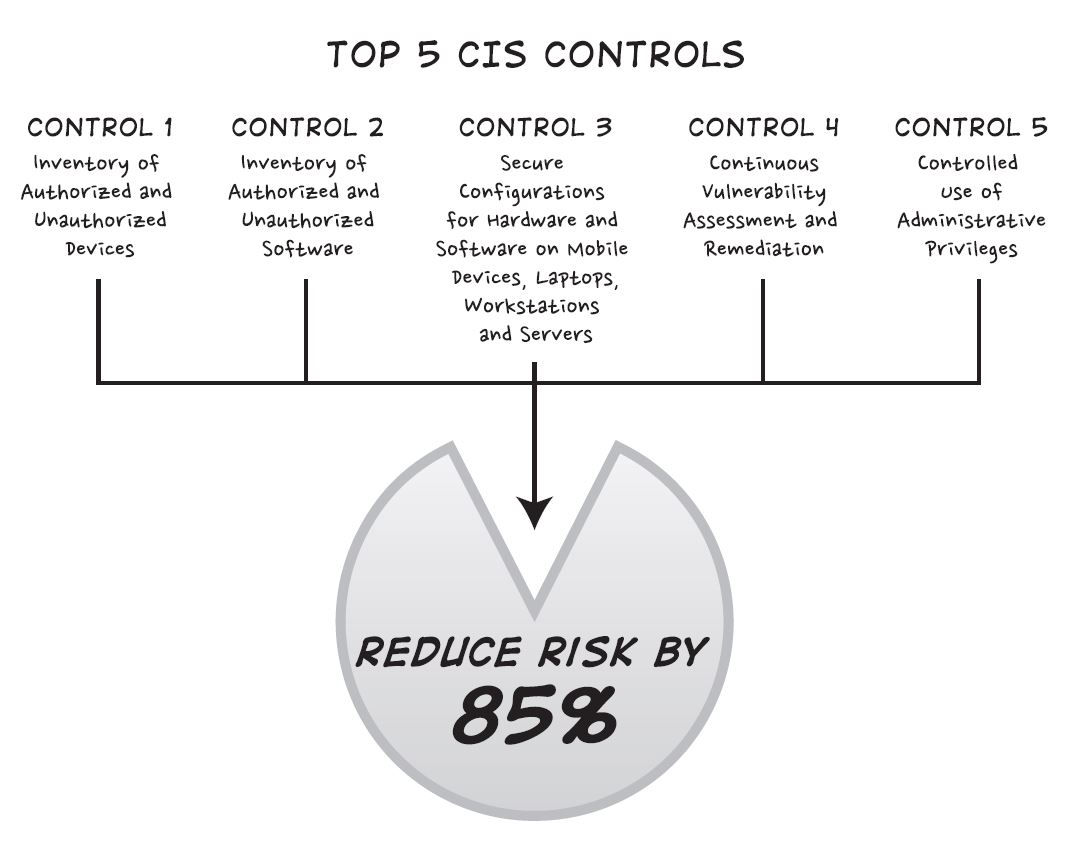
\includegraphics[scale=0.45]{./figures/fig6.jpg}
\caption{The ``Top 5 CIS Controls'' can stop 85 percent of cyberattacks.}
\label{fig:Fig2}
\end{figure}
\vspace{10pt}

\begin{formal}
    
\begin{quote} 
\begin{minipage}{\linewidth}
\stepcounter{footnote}
\renewcommand\thempfootnote{\textcolor{orange}{\arabic{footnote}}}

In cybersecurity, there are five controls that stop 85 percent of all attacks.\footnote{``The 20 CIS Controls \& Resources,'' Center for Internet Security, accessed October 20,2020, 
\url{https://www.cisecurity.org/controls/cis-controls-list/}.}
\vspace{10pt}

If these five controls stop 85 percent of attacks, does it make sense to spend time on anything else until you've mastered them?\ Until these five controls are in place, does it make sense to focus on anything else?
\vspace{10pt}

One-hundred-item frameworks overcomplicate simple solutions, and often these five crucial controls are glossed over or ignored.

\hfill
---\cite{Espinosa2021-is}
\end{minipage}
\end{quote}
\end{formal}

Along with the excerpt shown above, Figure \ref{fig:Fig2} can be found on page 41 of Christian Espinosa's book (listed in the bibliography as entry 5). The source file (.jpg) was downloaded from the book's companion site, \url{https://christianespinosa.com/resources/tspitr/}. Since the book's time of publication (February of 2021), the number of CIS controls has been reduced to 18.

%% Include these options if you want the image to take up the entire page in portrait mode: 
%% [height=\textheight,width=.9\paperwidth]